% chap4.tex (Definitions and Theorem)

\chapter{Storage Optimization Framework for Provenance Data Storage in IoT} \label{MostNarrowEasy}

In this chapter, we optimize storage of provenance using our IoT provenance-collection framework.

%\section{Definitions}
%
%\begin{definition}
%{\rm We say that the number $\tilde x$ represents a number $x$ with
%{\em absolute accuracy\/} $\Delta>0$ if $|x-\tilde x|\leq\Delta$.}
%\end{definition}
%
%\begin{definition}
%{\rm By {\em absolute half-width\/} of the interval ${\bf x}=[x^-,x^+]$, we
%mean the smallest number $\Delta>0$ for which every number in ${\bf x}$ is
%represented with an absolute accuracy~$\Delta$ by $\tilde x=\displaystyle{
%\frac{x^-+x^+}{2}}$.\\[0.5pc]
%{\bf Proposition} It can be seen that the absolute half-width of ${\bf x}$ is
%$$
%  \max_{x\in [x^-,x^+]} |x-\tilde x| = \frac{x^+-x^-}{2}.
%$$}
%\end{definition}


\section{A Policy-Based Approach for Provenance Storage}
\par Provenance easily can generate more data than the size of the entity's data about  which provenance is being collected. Due to the large influx of real-time data generated from sensors and actuators in IoT, we anticipate large amounts of provenance data will be generated from our provenance collection framework. The resource constraints on the sensor-actuator and the device layer of the IoT architecture makes storing that data even more challenging. To address this challenge, we define a policy driven framework that provides a policy scheme for the optimization of provenance storage \textcolor{red}{and addresses resource constraints encountered when storing large amounts of provenance data.} Policy allows flexibility of provenance collection and pruning for a specific IoT application thereby eliminating irrelevant provenance data. Since organizations have varied provenance requirement(s), making a static provenance policy is not suitable for the IoT. Using policy for storage optimization is slightly different from the typical use of policy in enforcing access control. 



\textcolor{red}{ For the IoT framework, the product manufacturer is considered a policy creator. This reduces the complexity of creating and managing policy documents by the IoT device consumers. A policy creator is a user which has the right to add, delete or modify a policy document. A policy document is required to specify which provenance data to collect thereby providing storage access to provenance unlike system access control which evaluates user access rights to view a resource. }





\par 

\textcolor{red}{The policy framework consists of a policy engine. The policy engine contains authorization and enforcement components that provides and enforce decisions on how provenance data should be stored. }A policy document is a component of the policy framework. It identifies provenance data that is considered relevant to the IoT application. Our policy architecture is modeled using the Common Open Policy Service (COPS) Standard \cite{rfc2748}. COPS consists of components for policy generation, evaluation and enforcement. The Policy Enforcement Point (PEP) enforces decisions received from the Policy Decision Point (PDP). The PDP evaluates policies and generates decision based on the evaluation. The model can be extended to include a secondary decision point (SDP) which allows for distributed policy evaluation, thus freeing up the PDP from communication bottlenecks caused by large amounts of requests received by a single PDP.  

\par Figure \ref{policy_architecture} below illustrates the system architecture of our proposed policy-based storage framework. Different layers of the IoT architecture contain different decision and enforcement components. The sensor-actuator layer of the IoT architecture is omitted because it has negligible memory resources and the  sensors and actuators are usually physically part of a device in the device layer and as such does not have any data to prune. 

\begin{figure}[h!]
\begin{center}
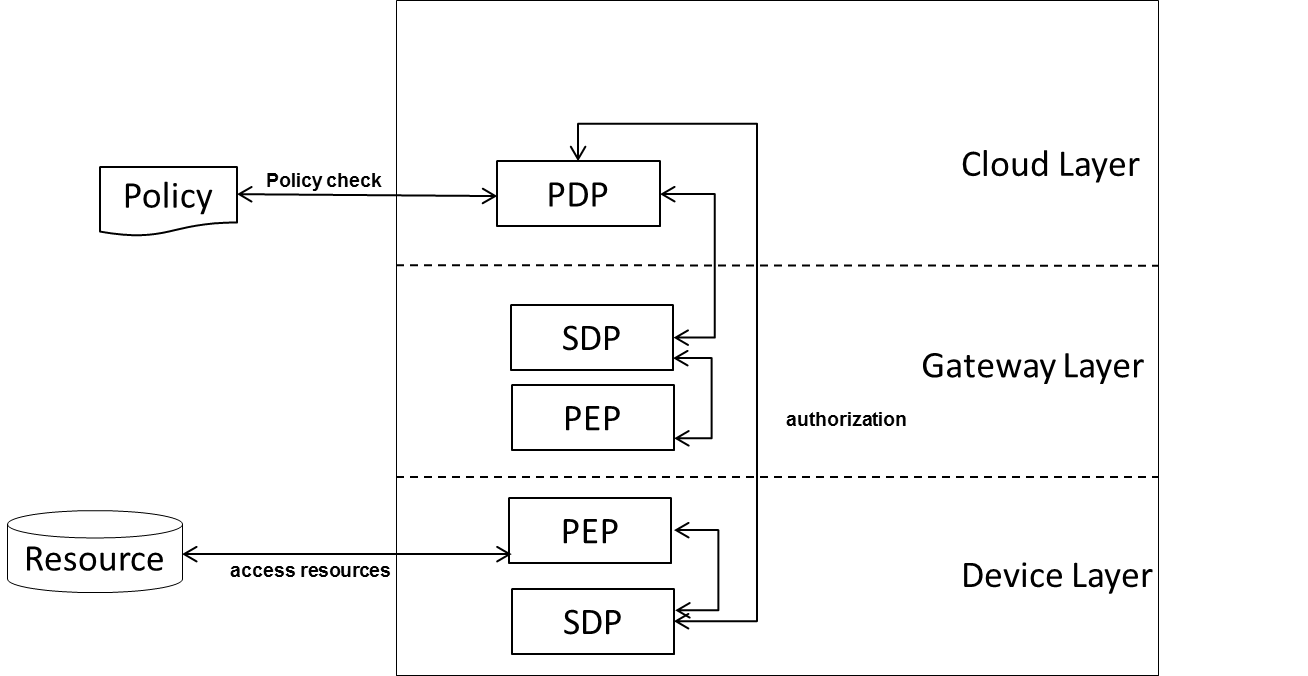
\includegraphics[height=3.5in]{policy.png}
\caption{Policy based system architecture which allows for effective data storage of provenance data}
\label{policy_architecture}
\end{center}
\end{figure}


Policy document which is generated by the policy creator serves as an input to the PDP component and is evaluated at the device, gateway and cloud layer. The PEP which is involved with generating requests is located in the device and gateway layer. SDPs can be located in the gateway layer, which allows for policy evaluation without inuring additional network overhead of communicating with the PDP located in the cloud layer. 


%% you removed the XACML section from here.

\par Using the use case of the smart home depicted in chapter 2, a policy framework could be implemented and incorporated into the IoT which allows a device administrators to specify what kinds of provenance data to collect. The policy acts an enforcement point providing an efficient storage mechanism in a resource constrained environment. The contents of the implementation details for the policy framework which specifies the policy grammar and the policy architecture across the IoT stack are left as future work.


\section{Provenance Information Flow}

This section unifies components of our IoT provenance collection system. Figure \ref{flow_chart} depicts a flowchart which illustrates how provenance is generated and how the storage policy is used to enforce access on provenance data. Input data are represented in green while processes are represented by the blue rectangles. Policy document determines what kinds of provenance data to collect and store. The policy creator can be a device owner who has access and authority to the device. A yaml configuration file is passed as an input to the the tracer component. This contains the barectf application that collects CTF trace from sensor-actuator readings on the device. The yaml configuration is an essential portion of the tracer system.  It is used to generate application CTF trace output. It contains instructions of what trace data to collect. The policy framework takes a modular approach: policy component can be added at various layers of the IoT architecture. The policy engine is involved with the authorization and enforcement of policies generated. This portion generates a decision based on the policy evaluation. The response from the policy allows provenance effectively pruned. Provenance data stored as CTF trace in neo4j, a graph database and is mapped to PROV-JSON format. The PROV-JSON serialization is used as input to our IDS system which serves as the provenance application. Figure \ref{flow_chart} below illustrates the relationship between various component in the provenance aware IoT framework.

\begin{figure}[h!]
\begin{center}

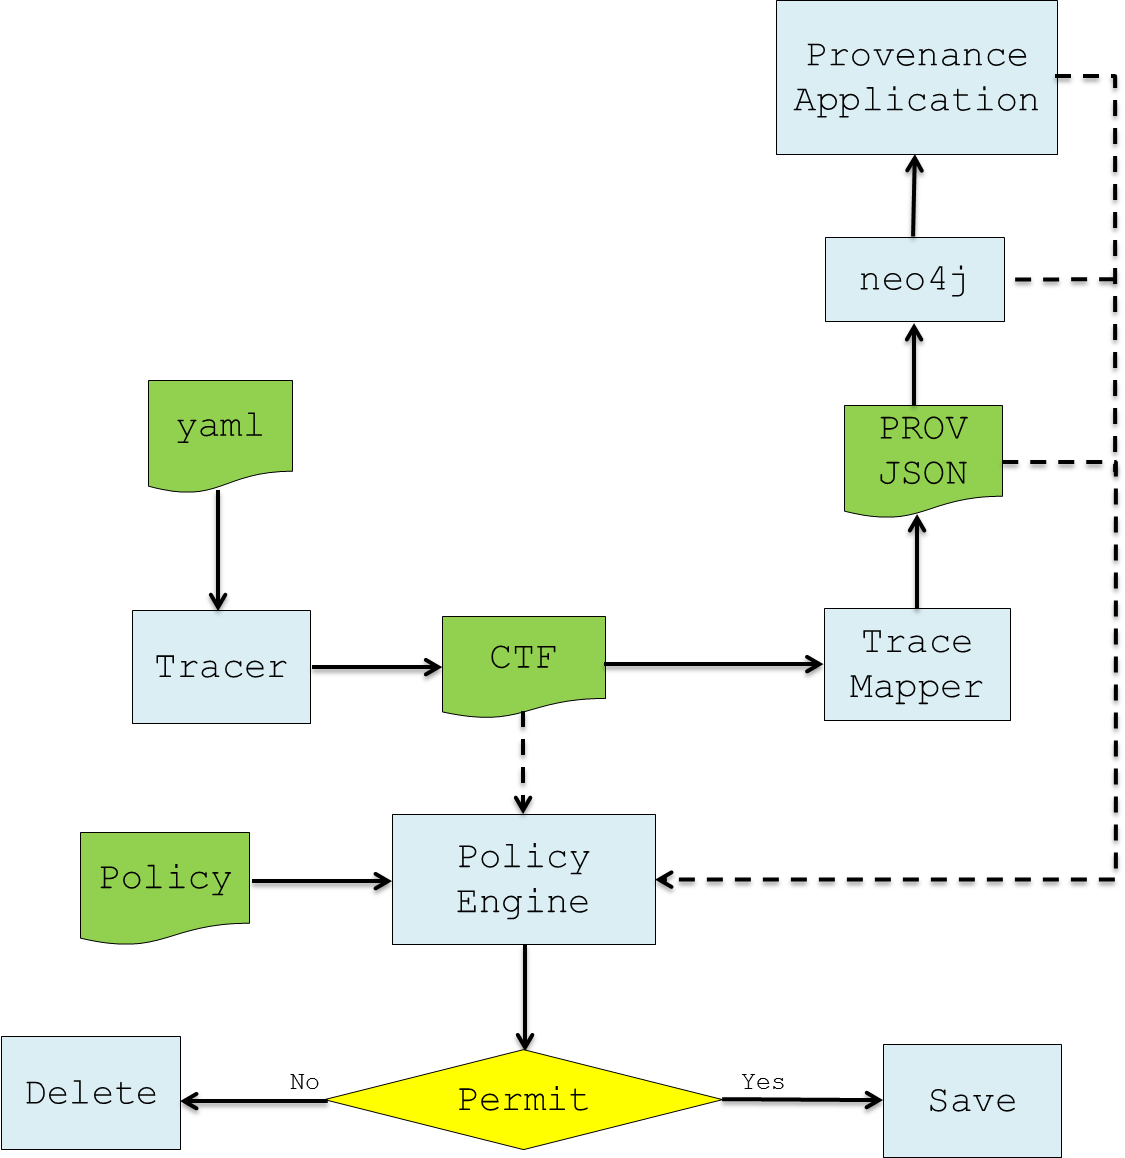
\includegraphics[width =4.5in]{policy_flowchart.PNG}    
\end{center}
\caption{Provenance Information Flowchart }
\label{flow_chart}
\end{figure}

\section{Policy-Based System}

In this section, I will explain various software tools in which I plan to use to implement a proof of concept for the policy-based storage system. Some of these tools have been illustrated in chapter 4. 


\par To map CTF trace to PROV-DM format, I plan to use babelctf, a plugin framework that allows converting from one trace format to another. PROV-DM data is represented in PROV-JSON serialized format and stored in a graph database. PROV-JSON is used as input to the provenance application which leverage provenance data to perform some application specific functionality. For our implementation, we choose to use a provenance-based IDS system.

%ProvToolbox, a java library for creating and visualizing provenance data. It also allows the conversion of provenance data from one format to another(e.g PROV-DM to PROV-JSON).

To implement our policy based framework, We plan to use the eXtensible Markup Language (XACML)  \cite{xacml} to generate an enforceable provenance storage policy for our IoT policy based system. XACML is a standard that defines constructs for policy language(i.e policy document, policy enforcement and policy authorization). We employ this standard in building our policy based system.


\subsection{Policy-Based Framework Evaluation}

To demonstrate the effectiveness of our framework, we implement a prototype for proof of concept. In order to collect sensor-actuator trace data, I plan to create a sample application implemented on a microcontroller. We chose an application that simulates a smart home lock authentication system. This system uses facial recognition to recognize and grant access to a door lock. I plan to implement this using a web camera attached to the microcontroller. On the microcontroller is contained OpenCV, an open source software library  developed for image processing. OpenCV allows for facial recognition on the microcontroller. Trace data generated from the smart home lock system in the form of CTF is collected on the microcontroller using barectf. CTF trace is translated to PROV-JSON which is stored in Neo4j, a graph database. Neo4j allows for querying and visualization of provenance. PROV-JSON is used as an input to the provenance application. For our implementation, we use a provenance based IDS, PIDAS as a provenance application that evaluates the effectiveness of our framework. The details of PIDAS is discussed in chapter 4. To evaluate PIDAS, we analyze the throughput and overhead incurred in addition to false negative and true positive as described in chapter 4.







%\section{Proposed Research Experiment Evaluation}
%
%We plan to evaluate the effectiveness of our approach for the provenance collection framework and our framework for efficient provenance storage by running an intusion detection system for IoT device. An IDS is used to detect malicious attacks based on a certain policy or thresehold set by an administrator. There are two types of  IDS: Rule-based apprach, or anomaly based apporach. The rule based approach allows for intrusion monitoring based on rules specified by an adminstrator. On the other hand, anomaly based IDS which monitors intrusion based on patterns that falls out of the normal system function. Most anomaly\-based approach deals with machine learning to classify normal or anomalous behaviour.  

%\begin{definition}
%{\rm By {\em absolute width\/} $W$ of an interval ${\bf x}=[x^-,x^+]$, we mean
%twice the absolute half-width of ${\bf x}$, i.e.,
%$$
%  W([x^-,x^+])=x^+-x^-.
%$$}
%\end{definition}
%
%\begin{definition}
%{\rm We say that an interval ${\bf x}$ is {\em $\Delta$-narrow in the sense
%of absolute accuracy\/} if $W({\bf x})\leq\Delta$.}
%\end{definition}
%
%\begin{definition}
%{\rm Let $\varepsilon>0$ be a real number, let $D\subseteq R^N$ be a closed
%and bounded set of positive $N$-dimension volume $V(D)>0$, and let
%$P(x)$ be a property that is true for some points $x\in D$.  We say that $P(x)$
%is true for {\em $(D,\varepsilon)$-almost all\/} $x$ if}
%$$
%  \frac{V(\{x\in D|\neg P(x)\})}{V(D)}\leq \varepsilon.
%$$
%\end{definition}
%
%\begin{definition}
%{\rm Let $\eta>0$ be a real number.  We say that intervals
%$$
%  [r_1-d_1,r_1+d_1],\ldots,[r_n-d_n,r_n+d_n]
%$$
%are {$\eta$-close} to intervals
%$$
%  [\tilde x_1-\Delta_1,\tilde x_1+\Delta_1],\ldots,[\tilde x_n-\Delta_n,
%   \tilde x_n+\Delta_n]
%$$
%if $|r_i-\tilde x_i|\leq\eta$ and 
%$|d_i-\Delta_i|\leq\eta$ for all $i$.}
%\end{definition}
%
%\begin{definition}
%{\rm Let $\cal U$ be an algorithm that solves some systems of interval linear
%equations, and let $\eta>0$ be a real number.  We say that an algorithm 
%$\cal U$ is {\em $\eta$-exact\/} for the interval matrices ${\bf a}_{ij}$ and
%${\bf b}_i$ if for every interval matrix ${\bf a}_{ij}^\prime$ and 
%${\bf b}_i^\prime$ that are $\eta$-close to ${\bf a}_{ij}$ and ${\bf b}_i$,
%the algorithm $\cal U$ returns the exact solution to the system}
%$$
%  \sum_{j=1}^n {\bf a}_{ij}^\prime x_j = {\bf b}_i^\prime.
%$$
%\end{definition}
%
%\begin{definition}
%{\rm We say that an algorithm $\cal U$ is {\em almost always exact for narrow 
%input intervals\/} if for every closed and bounded set $D\subseteq R^N
%(N=n\cdot m+n)$ there exist $\varepsilon>0$, $\Delta>0$ and $\eta>0$ such
%that, for $(D,\varepsilon)$-almost all $\tilde a_{ij}$ and $\tilde b_i$, if
%all input intervals ${\bf a}_{ij}$ and ${\bf b}_i$
%(containing $\tilde a_{ij}$ and $\tilde b_i$ respectively)
%are $\Delta$-narrow (in the sense of absolute accuracy), then the
%algorithm $\cal U$ is $\eta$-exact for ${\bf a}_{ij}$ and ${\bf b}_i$.}
%\end{definition}
%
%\section{Theorem}
%
%\begin{theorem} \label{almost-all-theorem}
%There exists a feasible (polynomial-time) algorithm $\cal U$ that is almost 
%always exact for narrow input intervals.
%\end{theorem}
%
%\medskip
%
%\noindent
%This theorem was proven in 1995 by Lakeyev and Kreinovich
%(see~\cite{Lakeyev1995}).
%
%\section{Open Problem}
%Theorem \ref{almost-all-theorem} says that we can have a feasible algorithm 
%that solves {\em almost all\/} narrow-interval linear equation systems, but 
%it does not say whether we can solve {\em all\/} of them in reasonable time.  
%Thus, there still remains an open question:
%
%\begin{quote}
%{\it Can a feasible algorithm be developed for the general problem of
%solving systems of linear equations with narrow-interval coefficients?}
%\end{quote}
%
%\noindent
%The answer to this open question is the main concern of this thesis.
%
%We will show that the problem of solving all narrow-interval linear equation
%systems is NP-hard; moreover, we will show that the problem is NP-hard not
%only for intervals that are narrow in the sense of absolute accuracy, but
%also in the sense of relative accuracy.

